\documentclass{article}

\usepackage[vmarginratio=1:1,a4paper,body={6.5in, 9.5in}]{geometry}

\usepackage[T2A]{fontenc}
\usepackage[utf8]{inputenc}
\usepackage[russian]{babel}

\usepackage{color}

\usepackage{amsmath}
\DeclareMathOperator*{\argmin}{arg\,min}

\usepackage{amssymb}
\usepackage{amsfonts}
\usepackage{amsthm}
\newtheorem{theorem}{Theorem}
\newtheorem{definition}{Definition}

\usepackage{hyperref}
\usepackage{graphicx}
\graphicspath{{./img/}}


\begin{document}

Итак продолжаем разговор о наименьших квадратах. В рамках этой статьи моим основным инструментом будет поиск минимума квадратичных функций; но, прежде чем мы начнём этим инструментом пользоваться, нужно хотя бы понять, где у него кнопка вкл/выкл.
Для начала освежим память и вспомним, что такое матрицы, что такое положительное число, а также что такое производная. 

\section{Матрицы и числа}
В этом тексте я буду обильно пользоваться матричными обозначениями, так что давайте вспоминать, что это такое. Не подглядывайте дальше по тексту, сделайте паузу на несколько секунд, и попробуйте сформулировать, что такое матрица.

\subsection{Различные интерпретации матриц}

Ответ очень простой. Матрица это просто шкафчик, в котором хранятся хреновины. Каждая хреновина лежит в своей ячейке, ячейки группируются рядами в строки и столбцы.
В нашем конкретном случае хреновинами будут обычные вещественные числа; для программиста проще всего представлять матрицу $A$ как нечто навроде \begin{verbatim}float A[m][n];\end{verbatim}

Зачем же такие хранилища нужны? Что они описывают? Может быть, я вас расстрою, но сама по себе матрица не описывает ничего, она хранит. Например, в ней можно хранить коэффициенты всяких функций.
Давайте на секунду забудем про матрицы, и представим, что у нас есть число $a$. Что оно означает?
Да чёрт его знает... Например, это может быть коэффициент внутри функции, которая на вход берёт одно число, и на выход даёт другое число:
$$
f(x) : \mathbb R \rightarrow \mathbb R
$$

Одну версию такой функции математик мог бы записать как 
$$
f(x) = ax
$$
Ну а в мире программистов она бы выглядела следующим образом:
\begin{verbatim}    
float f(float x) {
    return a*x;
}
\end{verbatim}

С другой стороны, а почему такая функция, а не совсем другая?
Давайте возьмём другую!
$$
f(x) = ax^2
$$
Раз уж я начал про программистов, я обязан записать её код :)
\begin{verbatim}    
float f(float x) {
    return x*a*x;
}
\end{verbatim}

Одна из этих функций линейная, а вторая квадратичная. Какая из них правильная? Да никакая, само по себе число $a$ не определяет этого, оно просто хранит какое-то значение! Какую вам надо функцию, такую и стройте.

То же самое происходит и с матрицами, это хранилища, нужные на случай, когда одиночных чисел (скаляров) не хватает, своего рода расширение чисел.  Над матрицами, ровно как и над числами, определены операции сложения и умножения. С делением чуть сложнее, но в определённых случаях и оно может быть определено.

Давайте представим, что у нас есть матрица $A$, например, размера 2x2:
$$
A=\begin{bmatrix} a_{11} & a_{12} \\ a_{21} & a_{22}\end{bmatrix}
$$

Эта матрица сама по себе ничего не значит, например, она может быть интерпретирована как функция
$$
f(x) : \mathbb R^2 \rightarrow \mathbb R^2, \quad f(x) = Ax
$$

\begin{verbatim}    
vector<float> f(vector<float> x) {
    return vector<float>{a11*x[0] + a12*x[1],  a21*x[0] + a22*x[1]};
}
\end{verbatim}

Эта функция преобразует двумерный вектор в двумерный вектор. Графически это удобно представлять как преобразование изображения: на вход даём изображение, а на выходе получаем его растянутую и/или повёрнутую (возможно даже зеркально отражённую!) версию.
Верхний ряд иллюстрации~\ref{fig:matrices} приводит различные примеры такой интерпретации матриц.


А можно матрицу $A$ представлять себе как функцию, которая двумерный вектор преобразует в скаляр:
$$
f(x) : \mathbb R^2 \rightarrow \mathbb R, \quad f(x) = x^\top A x = \sum\limits_i\sum\limits_j a_{ij}x_i x_j
$$

Обратите внимание, что с векторами возведение в степень не очень-то определено, поэтому я не могу написать $x^2$, как писал в случае с обычными числами. Очень рекомендую тем, кто не привык с лёгкостью жонглировать матричными умножениями, ещё раз вспомнить правило умножения матриц, и проверить, что выражение $x^\top A x$ вообще разрешено и действительно даёт скаляр на выходе.
Для этого можно, например, явно поставить скобки $x^\top A x = (x^\top A) x$
Напоминаю, что у нас $x$ - вектор размерности 2 (сохранённый в матрице размерности 2x1), выпишем явно все размерности:
$$
\underbrace{\underbrace{\left(\underbrace{x^\top}_{1\times 2} \times \underbrace{A}_{2\times 2}\right)}_{1\times 2} \times \underbrace{x}_{2\times 1}}_{1 \times 1}
$$

Возвращаясь в тёплый и пушистый мир программистов, мы можем записать эту же квадратичную функцию как-то так:
\begin{verbatim}    
float f(vector<float> x) {
    return x[0]*a11*x[0] + x[0]*a12*x[1] + x[1]*a21*x[0] + x[1]*a22*x[1];
}
\end{verbatim}

\begin{figure}[ht]
	\centering
	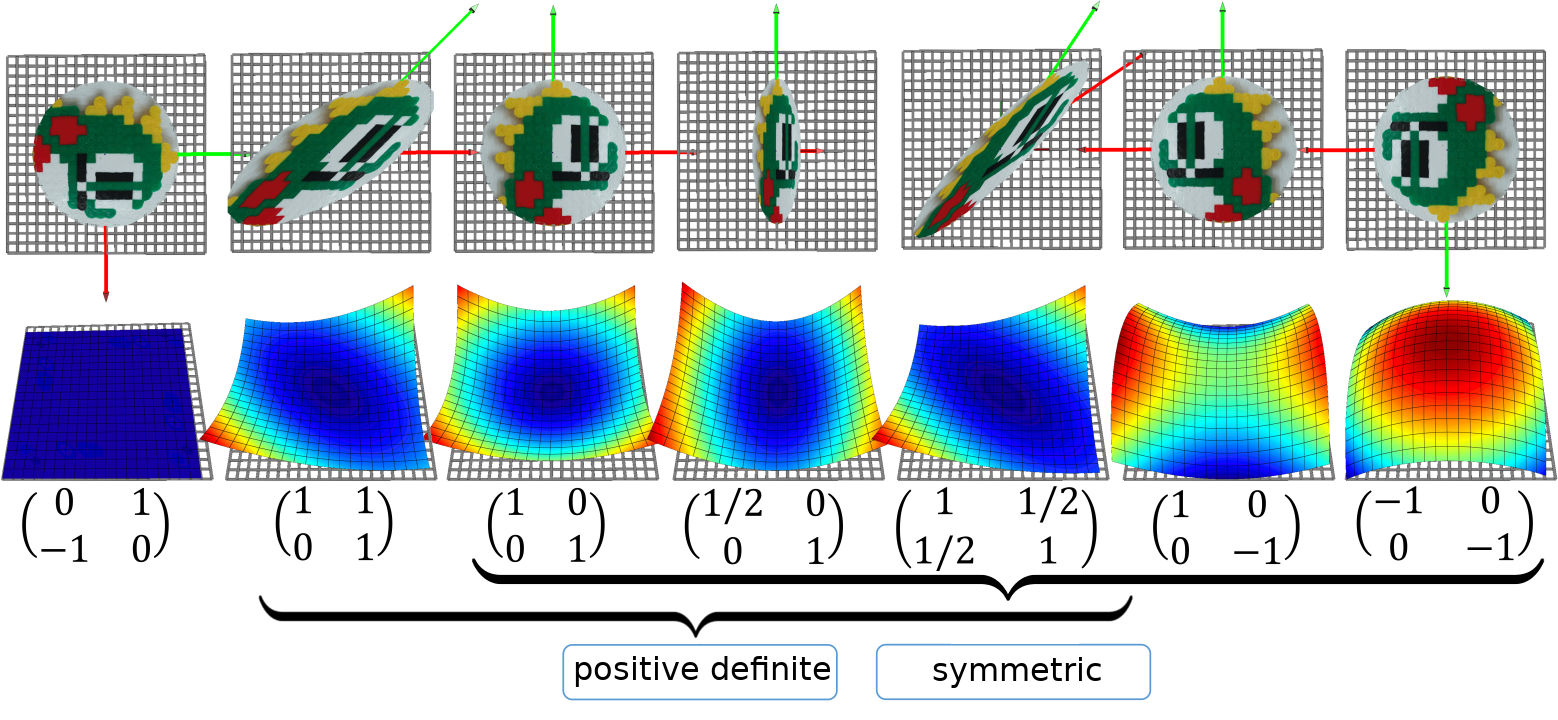
\includegraphics[width=\linewidth]{matrices}
	\caption{Семь примеров матриц $2\times 2$, как положительно определённых и симметричных, так и не очень. Верхний ряд: интерпретация матриц как функций $f(x):\mathbb R^2 \rightarrow \mathbb R^2$. Средний ряд: интерпретация матриц как функций $f(x):\mathbb R^2 \rightarrow \mathbb R$.}
	\label{fig:matrices}
\end{figure}


\subsection{Что такое положительное число?}
Теперь я задам очень глупый вопрос: что такое положительное число?
У нас есть отличный инструмент, называется предикат больше $>$.
Но не торопитесь отвечать, что число $a$ положительно тогда и только тогда, когда $a>0$, это было бы слишком просто. Давайте определим положительность следущим образом:
\begin{definition}
Число $a$ положительно тогда и только тогда, когда для всех ненулевых вещественных $x\in\mathbb R,\ x\neq 0$ выполняется условие $ax^2>0$.
\end{definition}

Выглядит довольно мудрёно, но зато отлично применяется к матрицам:

\begin{definition}
Квадратная матрица $A$ называется положительно определённой, если для любых ненулевых $x$
выполняется условие $x^\top A x > 0$, то есть, соответствующая квадратичная форма строго положительна везде, кроме начала координат.
\end{definition}

Для чего мне нужна положительность? Как я уже упоминал в начале статьи, моим основным инструментом
будет поиск минимумов квадратичных функций. А ведь для того, чтобы минимум искать, было бы недурно, если бы он существовал! Например, у функции $f(x) = - x^2$ минимума очевидно не существует, посколькуо число -1 не является положительным, и $f(x)$ бесконечно убывает с ростом $x$: ветви параболы $f(x)$ смотрят вниз.
Положительно определённые матрицы хороши тем, что соответствующие квадратичные формы образуют параболоид, имеющие (единственный) минимум. Иллюстрация~\ref{fig:matrices} показывает семь различных примеров матриц.

Таким образом, я буду работать с положительно определёнными матрицами, которые являются обобщением положительных чисел. Более того, конкретно в моём случае матрицы будут ещё и симметричными!
Любопытно, что довольно часто, когда люди говорят про положительную определённость, они подразумевают ещё и симметричность, что может быть косвенно объяснено следующим (необязательным для понимания последующего текста) наблюдением.

\subsubsection{Лирическое отступление о симметричности матриц квадратичных форм}

Давайте рассмотрим квадратичную форму $x^\top M x$ для произвольной матрицы $M$; затем
к $M$ добавим и сразу же отнимем половину её транспонированной версии:
$$
M = \underbrace{\frac{1}{2} (M+M^\top)}_{:=M_s} + \underbrace{\frac{1}{2} (M-M^\top)}_{:=M_a} = M_s + M_a
$$

Матрица $M_s$ симметрична: $M_s^\top = M_s$; матрица $M_a$ антисимметрична: $M_a^\top=-M_a$.
Примечательным фактом является то, что для любой антисимметричной матрицы соответствующая квадратичная форма тождественно равна нулю. Это вытекает из следующего наблюдения:
$$
q = x^\top M_a x  = (x^\top M_a^\top x)^\top = - (x^\top M_a x)^\top = -q
$$
То есть, квадратичная форма $x^\top M_a x$ одновременно равна $q$ и $-q$, что возможно только в том случае, когда $q\equiv 0$.
Из этого факта вытекает то, что для произвольной матрицы $M$ соответствующая  квадратичная форма $x^\top M x$ может быть выражена и через симметричную матрицу $M_s$:
$$
x^\top M x = x^\top (M_s + M_a) x = x^\top M_s x  + x^\top M_a x = x^\top M_s x.
$$


\section{Ищем минимум квадратичной функции}

\begin{figure}[ht]
	\centering
	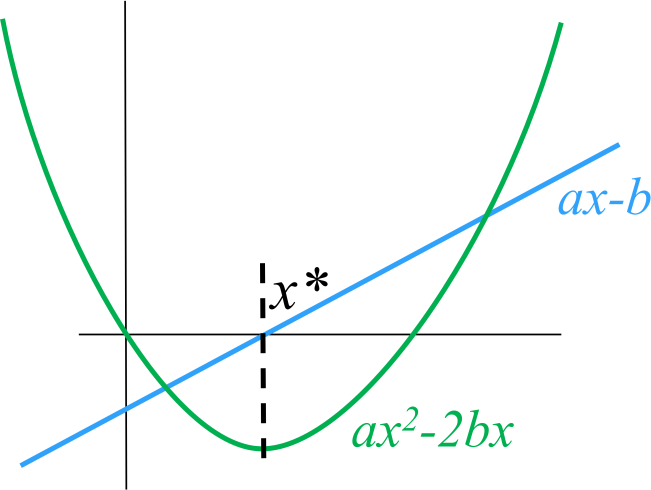
\includegraphics[width=.3\linewidth]{minpb1d}
	\caption{В одномерном мире решение $x^*$ уравнения $ax - b = 0$ также является решением проблемы $\argmin\limits_x(ax^2-2bx)$. }
	\label{fig:min1d}
\end{figure}

Вернёмся ненадолго в одномерный мир; я хочу найти минимум функции $f(x) = ax^2 - 2bx$. Число $a$ положительно, поэтому минимум существует; чтобы его найти, приравняем нулю соответствующую производную: $\frac{d}{dx}f(x) = 0$. Продифференцировать одномерную квадратичную функцию труда не составляет: $\frac{d}{dx}f(x) = 2ax - 2b = 0$; поэтому наша проблема сводится к решению уравнения $ax-b=0$, откуда
путём страшных усилий получам решение $x^* = b/a$. Рисунок~\ref{fig:min1d} иллюстрирует эквивалентность двух проблем: решение $x^*$ уравнения $ax-b=0$ совпадает с решением уравнения $\argmin\limits_x(ax^2 - 2bx)$.

Я клоню к тому, что нашей глобальной целью является минимизация квадратичных функций, мы же про наименьшие квадраты говорим. Но при этом что мы действительно умеем делать хорошо, так это решать линейные уравнения (и системы линейных уравнений). И очень здорово, что одно эквивалентно другому!
Единственное, что нам осталось, так это убедиться, что эта эквивалентность в одномерном мире распространяется и на случай $n$ переменных. Чтобы это проверить, для начала докажем три теоремы.

\subsection{Три теоремы, или дифференцируем матричные выражения}
Первая теорема гласит о том, что матрицы $1\times 1$ инварианты относительно транспонирования:
\begin{theorem}
$x\in \mathbb R \Rightarrow x^\top = x$
\end{theorem}
Доказательство настолько сложное, что для краткости я вынужден его опустить, но попробуйте найти его самостоятельно.

Вторая теорема позволяет дифференцировать линейные функции. В случае вещественной функции одной переменной мы знаем, что $\frac{d}{dx}(bx) = b$, но что происходит в случае вещественной функции $n$ переменных?
\begin{theorem}
$\nabla b^\top x = \nabla x^\top b = b$
\end{theorem}
То есть, никаких сюрпризов, просто матричная запись того же самого школьного результата. Доказательство крайне прямолинейное, достаточно просто записать определение градиента:
$$\nabla(b^\top x) = \begin{bmatrix}\frac{\partial (b^\top x)}{\partial x_1} \\ \vdots \\ \frac{\partial (b^\top x)}{\partial x_n} \end{bmatrix} = \begin{bmatrix}\frac{\partial (b_1 x_1 + \dots + b_n x_n)}{\partial x_1} \\ \vdots \\ \frac{\partial (b_1 x_1 + \dots + b_n x_n)}{\partial x_n} \end{bmatrix}
= \begin{bmatrix}b_1 \\ \vdots \\ b_n \end{bmatrix} = b$$
Применив первую теорему $b^\top x = x^\top b$, мы завершаем доказательство.

Теперь переходим к квадратичным формам. Мы знаем, что в случае вещественной функции одной переменной $\frac{d}{dx}(ax^2) = 2ax$, а что будет в случае квадратичной формы?
\begin{theorem}
$\nabla (x^\top A x) = (A+A^\top)x$
\end{theorem}
Кстати, обратите внимание, что если матрица $A$ симметрична, то теорема гласит, что $\nabla (x^\top A x) = 2Ax$.

Это доказательство тоже прямолинейно, просто запишем квадратичную форму как двойную сумму:
$$x^\top A x = \sum\limits_i\sum\limits_j a_{ij} x_i x_j$$
А затем посмотрим, чему равна частная производная этой двойной суммы по переменной $x_i$:
\begin{align*}
\frac{\partial (x^\top A x)}{\partial x_i} 
&= \frac{\partial}{\partial x_i}  \left(\sum\limits_{k_1}\sum\limits_{k_2} a_{k_1 k_2} x_{k_1} x_{k_2}\right) = \\
&= \frac{\partial}{\partial x_i}  \left(
\underbrace{\sum\limits_{k_1\neq i}\sum\limits_{k_2\neq i} a_{ik_2}x_{k_1} x_{k_2}}_{k_1 \neq i, k_2 \neq i}+\underbrace{\sum\limits_{k_2\neq i} a_{ik_2}x_i x_{k_2}}_{k_1 = i, k_2\neq i}+
\underbrace{\sum\limits_{k_1\neq i} a_{k_1 i} x_{k_1} x_i}_{k_1 \neq i, k_2 = i}+
\underbrace{a_{ii}x_i^2}_{k_1 = i, k_2 = i}\right) = \\
& = \sum\limits_{k_2\neq i} a_{ik_2}x_{k_2} + \sum\limits_{k_1\neq i} a_{k_1 i} x_{k_1} + 2 a_{ii} x_i = \\
& = \sum\limits_{k_2} a_{ik_2}x_{k_2} + \sum\limits_{k_1} a_{k_1 i} x_{k_1} = \\
& = \sum\limits_{j} (a_{ij} + a_{ji}) x_j \\
\end{align*}
Я разбил двойную сумму на четыре случая, которые выделены фигурными скобками. Каждый из этих четырёх случаев дифференцируется тривиально. Осталось сделать последнее действие, собрать частные производные в вектор градиента:
$$\nabla(x^\top A x) = \begin{bmatrix}\frac{\partial (x^\top Ax)}{\partial x_1} \\ \vdots \\ \frac{\partial (x^\top A x)}{\partial x_n} \end{bmatrix}  = \begin{bmatrix}\sum\limits_{j} (a_{1j} + a_{j1}) x_j \\ \vdots \\ \sum\limits_{j} (a_{nj} + a_{jn}) x_j \end{bmatrix}  = (A+A^\top)x
$$

\subsection{Минимум квадратичной функции и решение линейной системы}
Давайте не забывать направление движения. Мы видели, что при положительном числе $a$ в случае вещественных функций одной перменной решить уравнение $ax=b$ или минимизировать квадратичную функцию $\argmin\limits_x(ax^2 - 2bx)$ --- это одно и то же.

Мы хотим показать соответствующую связь в случае симметричной положительно определённой матрицы $A$.
Итак, мы хотим найти минимум квадратичной функции 
$$\argmin\limits_{x\in\mathbb R^n} (x^\top A x - 2b^\top x).$$
Ровно как и в школе, приравняем нулю производную:
$$\nabla (x^\top A x - 2b^\top x) = \begin{bmatrix}0 \\ \vdots \\ 0 \end{bmatrix}.$$
Оператор Гамильтона линеен, поэтому мы можем переписать наше уравнение в следующем виде:
$$\nabla (x^\top A x) - 2\nabla(b^\top x) = \begin{bmatrix}0 \\ \vdots \\ 0 \end{bmatrix}$$
Теперь применим вторую и третью теоремы о дифференцировании:
$$(A+A^\top)x - 2b = \begin{bmatrix}0 \\ \vdots \\ 0 \end{bmatrix}$$
Вспомним, что $A$ симметрична, и поделим уравнение на два, получаем нужную нам систему линейных уравнений:
$$Ax = b$$
Ура-ура, перейдя от одной переменной к многим, мы не потеряли ровным счётом ничего, и можем эффективно минимизировать квадратичные функции!

%$$\argmin (x^\top A x - 2b^\top x) = A^{-1}b$$

\section{Переходим к наименьшим квадратам}
Наконец мы можем перейти к основному содержанию этой лекции. Представьте, что у нас есть две точки на плоскости $(x_1, y_1)$ и $(x_2, y_2)$, и мы хотим найти уравнение прямой, проходящей через эти две точки.
Уравнение прямой можно записать в виде $y = \alpha x + \beta$, то есть, наша задача это найти коэффициенты $\alpha$ и $\beta$. Это упражнение для седьмого-восьмого класса школы, запишем систему уравнений:
$$
\left\{
\begin{split}
\alpha x_1 + \beta &= y_1\\
\alpha x_2 + \beta &= y_2\\
\end{split}
\right.
$$

У нас два уравнения с двумя неизвестными ($\alpha$ и $\beta$), остальное известно.
В общем случае решение существует и единственно. Для удобства перепишем ту же самую систему в матричном виде:
$$
\underbrace{\begin{bmatrix}x_1  & 1 \\ x_2 & 1 \end{bmatrix}}_{:=A} 
\underbrace{\begin{bmatrix} \alpha \\ \beta \end{bmatrix}}_{:=x} = \underbrace{\begin{bmatrix} y_1 \\ y_2 \end{bmatrix}}_{:=b}
$$

Получим уравнение типа $Ax = b$, которое тривиально решается $x^* = A^{-1}b$.

А теперь представим, что у нас есть \textbf{три} точки, через которые нужно провести прямую:
$$
\left\{
\begin{split}
\alpha x_1 + \beta &= y_1\\
\alpha x_2 + \beta &= y_2\\
\alpha x_3 + \beta &= y_3\\
\end{split}
\right.
$$

В матричном виде эта система запишется следующим образом:
$$
\underbrace{\begin{bmatrix}x_1  & 1 \\ x_2 & 1 \\x_3 & 1 \end{bmatrix} }_{:= A\,(3\times 2)}
\underbrace{\begin{bmatrix} \alpha \\ \beta \end{bmatrix}}_{:=x\,(2\times 1)} = \underbrace{\begin{bmatrix} y_1 \\ y_2 \\ y_3 \end{bmatrix}}_{:=b\, (3\times 1)}
$$
Теперь у нас матрица $A$ прямоугольная, и у неё просто не существует обратной! Это совершенно нормально, так как у нас всего две переменных и три уравнения, и в общем случае эта система не имеет решения.
Это соверешенно нормальная ситуация в реальном мире, когда точки - это данные зашумлённых измерений, и нам нужно найти параметры $\alpha$ и $\beta$, которые наилучшим образом \textit{приближают} данные измерений.
Мы этот пример уже рассматривали в первой лекции, когда калибровали безмен. Но тогда у нас решение было чисто алгебраическим и очень громоздким. Давайте попробуем более интуитивный способ.

Нашу систему можно записать в следующем виде:
$$
\alpha \underbrace{\begin{bmatrix}x_1  \\ x_2 \\x_3  \end{bmatrix} }_{:=\vec{i}}
+\beta \underbrace{\begin{bmatrix}1 \\ 1 \\1 \end{bmatrix} }_{:=\vec{j}} = 
\begin{bmatrix}y_1\\y_2\\y_3\end{bmatrix}
$$
Или, более кратко, 
$$
\alpha \vec{i} + \beta\vec{j} = \vec{b}.
$$
Векторы $\vec i$, $\vec j$ и $\vec b$ известны, нужно найти скаляры $\alpha$ и $\beta$.
Очевидно, что линейная комбинация $\alpha \vec{i} + \beta\vec{j}$ порождает плоскость, и если вектор $\vec b$ в этой плоскости не лежит, то точного решения не существует; однако же мы ищем приближённое решение.

Давайте определим ошибку решения как $\vec{e}(\alpha, \beta) :=  \alpha \vec{i} + \beta\vec{j} - \vec b$.
Нашей зачей является найти такие значения параметров $\alpha$ и $\beta$, которые минимизируют длину вектора $\vec{e}(\alpha, \beta)$. Иначе говоря, проблема записывается как $\argmin\limits_{\alpha, \beta} \|\vec{e}(\alpha, \beta)\|$.
Иллюстрация дана на рисунке~\ref{fig:error}.

\begin{figure}[ht]
	\centering
	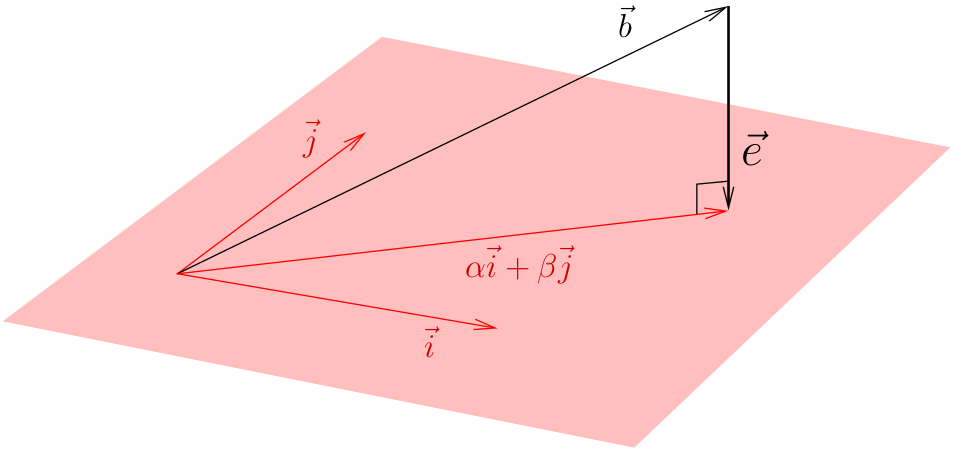
\includegraphics[width=.7\linewidth]{error}
	\caption{Имея заданные векторы $\vec i$, $\vec j$ и $\vec b$, мы стараемся минимизировать длину вектора ошибки $\vec e$. Очевидно, что его длина минимизируется, если он перпендикулярен плоскости, натянутой на векторы $\vec i$ и $\vec j$.}
	\label{fig:error}
\end{figure}

Но постойте, где же наименьшие квадраты? Сейчас будут. Функция извлечения корня $\sqrt{\cdot}$ монотонна, поэтому $\argmin\limits_{\alpha, \beta} \|\vec{e}(\alpha, \beta)\|$ = $\argmin\limits_{\alpha, \beta} \|\vec{e}(\alpha, \beta)\|^2$!

Вполне очевидно, что длина вектора ошибки минимизируется, если он перпендикулярен плоскости, натянутой на векторы $\vec i$ и $\vec j$, что можно записать, приравняв нулю соответствующие скалярные произведения:

$$
\left\{
\begin{split}\vec{i}^\top \vec{e}(\alpha, \beta) &= 0\\
\vec{j}^\top \vec{e}(\alpha, \beta) &= 0
\end{split}
\right.
$$

В матричном виде эту же самую систему можно записать как
$$
\begin{bmatrix}x_1 & x_2 & x_3 \\ 1 & 1 & 1 \end{bmatrix}
\left(\alpha \begin{bmatrix}x_1  \\ x_2 \\x_3  \end{bmatrix}
+\beta \begin{bmatrix}1 \\ 1 \\1 \end{bmatrix} - 
\begin{bmatrix}y_1\\y_2\\y_3\end{bmatrix}\right) = \begin{bmatrix}0\\0\end{bmatrix}
$$
или же
$$
\begin{bmatrix}x_1 & x_2 & x_3 \\ 1 & 1 & 1 \end{bmatrix}
\left(
\begin{bmatrix}x_1  & 1 \\ x_2 & 1 \\x_3 & 1 \end{bmatrix}
\begin{bmatrix} \alpha \\ \beta \end{bmatrix}-
\begin{bmatrix} y_1 \\ y_2 \\ y_3 \end{bmatrix}
\right) = \begin{bmatrix}0\\0\end{bmatrix}
$$
Но мы на этом не остановимся, так как запись можно ещё больше сократить:
$$
A^\top (Ax - b)= \begin{bmatrix}0\\0\end{bmatrix}
$$
И самая последняя трансформация:
$$
A^\top Ax = A^\top b.
$$
Давайте посчитаем размерности. Матрица $A$ имеет размер $3\times 2$, поэтому $A^\top A$ имеет размер $2\times 2$. Матрица $b$ имеет размер $3\times 1$, но вектор $A^\top b$ имеет размер $2\times 1$.
То есть, в общем случае матрица $A^\top A$ обратима! Более того, $A^\top A$ имеет ещё пару приятных свойств.

\begin{theorem}
$A^\top A$ симметрична.
\end{theorem}
Это совсем нетрудно показать:
$$
(A^\top A)^\top = A^\top (A^\top)^\top = A^\top A.
$$

\begin{theorem}
	$A^\top A$ положительно полуопределена: $\forall x\in \mathbb R^n\quad x^\top A^\top A x \geq 0.$
\end{theorem}
Это следует из того факта, что $x^\top A^\top A x = (A x)^\top A x > 0$.

Кроме того, $A^\top A$ положительно определена в том случае, если $A$ имеет линейно независимые столбцы (ранг $A$ равен количеству переменных в системе).

\vspace{5mm}

Итого, для системы с двумя неизвестными мы доказали, что минимизация 
квадратичной функции $\argmin\limits_{\alpha, \beta} \|\vec{e}(\alpha, \beta)\|^2$ эквивалентна решению системы линейных уравнений $A^\top A x = A^\top b$. Разумеется, всё это рассуждение применимо и к любому другому количеству переменных, но давайте ещё раз компактно запишем всё вместе простым алгебраическим подсчётом.
Мы начнём с проблемы наименьших квадратов, придём к минимизации квадратичной функции знакомого нам вида,
и из этого сделаем вывод об эквивалентности решению системы линейных уравнений. Итак, поехали:
\begin{align*}
\argmin \| Ax - b \|^2 &= \argmin (Ax-b)^\top (Ax-b) =\\
& = \argmin(x^\top A^\top - b^\top)(Ax-b) = \\
& = \argmin(x^\top A^\top A x - b^\top Ax - x^\top A^\top b + \underbrace{b^\top b}_{\rm const})=\\
& = \argmin(x^\top A^\top A x - 2b^\top Ax) = \\
& = \argmin(x^\top \underbrace{(A^\top A)}_{:=A'} x - 2\underbrace{(A^\top b)}_{:=b'}\phantom{}^\top x)
\end{align*}
Таким образом, проблема наименьших квадратов $\argmin \| Ax - b \|^2$  эквивалентна минимизации квадратичной функции $\argmin (x^\top A' x - 2b'^\top x)$ с (в общем случае) симметричной положительно определённой матрицей $A'$, что, в свою очередь, эквивалентно решению системы линейных уравнений $A'x = b'$. Уфф. Теория закончилась.
\end{document}
